% =====================================================================
% EE 269 Paper Presentation - Team 3
% Paper: A Survey on Data Selection for Language Models
% Authors: Joel Borja, Changxin Wan, Xingran Huang
% Published: Transactions on Machine Learning Research, 07/2024
%
% Every claim on every slide is sourced from the paper.
% Citation comments at the end of each frame use the format:
% % SOURCE: Section X, original text "..."
% =====================================================================

\documentclass[aspectratio=169]{beamer}

% ---------- Packages ----------
\usepackage[utf8]{inputenc}
\usepackage{amsmath, amssymb}
\usepackage{graphicx}
\usepackage{booktabs}
\usepackage{array}
\usepackage{xcolor}
\usepackage{tikz}
\usetikzlibrary{arrows.meta,positioning,fit,calc}

% ---------- Theme ----------
\usetheme{default}
\usecolortheme{default}
\setbeamertemplate{navigation symbols}{}
\setbeamertemplate{footline}[frame number]

% UCR colors
\definecolor{ucrblue}{RGB}{0, 64, 152}
\definecolor{ucrgold}{RGB}{255, 184, 28}
\definecolor{softblue}{RGB}{232, 241, 252}
\definecolor{softgold}{RGB}{255, 247, 224}
\definecolor{softgray}{RGB}{245, 246, 248}
\definecolor{methodgreen}{RGB}{26, 115, 92}
\definecolor{methodorange}{RGB}{194, 93, 34}
\definecolor{methodred}{RGB}{164, 54, 42}

\tikzset{
  methodbox/.style={
    draw=ucrblue,
    rounded corners=2pt,
    fill=softblue,
    align=center,
    inner sep=5pt,
    font=\small
  },
  methodarrow/.style={
    -{Latex[length=2.5mm]},
    thick,
    draw=ucrblue
  },
  riskbox/.style={
    draw=methodred,
    rounded corners=2pt,
    fill=red!6,
    align=center,
    inner sep=5pt,
    font=\small
  }
}

\setbeamercolor{frametitle}{fg=ucrblue}
\setbeamercolor{title}{fg=white}
\setbeamercolor{author}{fg=white}
\setbeamercolor{institute}{fg=white}

% Title page background
\setbeamertemplate{title page}{
  \begin{tikzpicture}[remember picture, overlay]
    \fill[ucrblue] (current page.south west) rectangle (current page.north east);
  \end{tikzpicture}
  \vfill
  \begin{center}
    {\color{white}\Large\bfseries \inserttitle\par}
    \vspace{1em}
    {\color{white}\insertauthor\par}
    {\color{white}\insertinstitute\par}
    {\color{white}\insertdate\par}
  \end{center}
  \vfill
}

\setbeamertemplate{itemize item}{$\bullet$}
\setbeamertemplate{itemize subitem}{$\circ$}

\title{Data Selection for LLMs}
\author{Paper Presentation \\ Joel Borja, Changxin Wan, Xingran Huang}
\institute{EE 269, UC Riverside}
\date{May 21, 2026}

\begin{document}

% =====================================================================
% Slide 1: Title
% =====================================================================
\begin{frame}[plain]
  \titlepage
\end{frame}
% SOURCE: Paper title page, "A Survey on Data Selection for Language Models", TMLR 07/2024.

% =====================================================================
% Slide 2: Presentation Roadmap / Agenda
% =====================================================================
\begin{frame}{Presentation Roadmap}

\vspace{1.5em}

\begin{columns}[T,totalwidth=\textwidth]

\begin{column}{0.31\textwidth}
\begin{minipage}[t][1.25cm][t]{\linewidth}
{\color{ucrblue}\large\textbf{1. Foundations \&\\ Motivation}}
\end{minipage}

\textbf{Joel Borja}

\vspace{0.8em}
Motivation, taxonomy, and the LLM data pipeline
\end{column}

\begin{column}{0.31\textwidth}
\begin{minipage}[t][1.25cm][t]{\linewidth}
{\color{ucrblue}\large\textbf{2. Methods \&\\ Techniques}}
\end{minipage}

\textbf{Changxin Wan}

\vspace{0.8em}
Filtering, deduplication, scoring, and sampling
\end{column}

\begin{column}{0.31\textwidth}
\begin{minipage}[t][1.25cm][t]{\linewidth}
{\color{ucrblue}\large\textbf{3. Applications \&\\ Future}}
\end{minipage}

\textbf{Xingran Huang}

\vspace{0.8em}
Applications, benchmarks, results, and future directions
\end{column}

\end{columns}

\vfill

\centering
\footnotesize
\textit{20 min presentation + 5 min Q\&A per section}
\quad --- \quad
\textit{5-minute break after Section 2}

\end{frame}
% \begin{frame}{Presentation Roadmap}
%   \textbf{What is multiported memory?}
%   \begin{itemize}
%     \item Memory that allows multiple concurrent reads and writes
%     \item Used to achieve high memory bandwidth in digital designs on FPGAs
%   \end{itemize}

%   \vspace{0.5em}
%   \textbf{Real applications on FPGA}
%   \begin{itemize}
%     \item Register file of MIPS like soft processors (1 write, 2 reads)
%     \item Shared cache among multiple soft processors
%     \item Routing table in network switching functions
%   \end{itemize}

%   \vspace{0.5em}
%   \textbf{The hardware reality}
%   \begin{itemize}
%     \item FPGAs use BRAMs (Block RAMs) as efficient memory blocks
%     \item A BRAM only natively supports 2 access ports
%     \item Building memory with more ports requires extra design effort
%   \end{itemize}
% \end{frame}

% =====================================================================
% Slide 3: Divider Slide for Foundations and Motivation
% =====================================================================
\begin{frame}

\begin{center}

\vspace{2cm}

{\color{ucrblue}\Huge\textbf{Part 1}}

\vspace{0.8cm}

{\LARGE Foundations \& Motivation}

\vspace{1cm}

{\large Data Selection for LLMs}

\end{center}

\end{frame}
% =====================================================================
% Slide 3: Why Data Matters for LLMs
% =====================================================================
\begin{frame}{Why Data Matters for LLMs}
  \begin{columns}[T]
    \begin{column}{0.55\textwidth}
      \textbf{Three previous techniques (Section II)}
      \begin{itemize}
        \item \textbf{Replication}: duplicate BRAMs to add read ports
        \item \textbf{LVT}: track latest value to add write ports
        \item \textbf{XOR based}: encode/decode with XOR for writes
      \end{itemize}

      \vspace{0.5em}
      \textbf{The gap}
      \begin{itemize}
        \item Can occupy more than half of available BRAMs on modern FPGAs
        \item Excessive BRAM usage blocks other parts of the design
        \item Complex routing limits operating frequency
      \end{itemize}

      \vspace{0.3em}
      \textit{$\rightarrow$ Need a more BRAM efficient design}
    \end{column}
    \begin{column}{0.45\textwidth}
      \centering
      % \includegraphics[width=\linewidth]{figures1/table1_techniques.png}
    \end{column}
  \end{columns}
\end{frame}

% =====================================================================
% Slide #: Questions
% =====================================================================
\begin{frame}

\begin{center}

\vspace{2.5cm}

{\color{ucrblue}\Huge\textbf{Questions?}}

\end{center}

\end{frame}

% =====================================================================
% Slide #: BREAK
% =====================================================================
\begin{frame}

\begin{center}

\vspace{2cm}

{\color{ucrblue}\Huge\textbf{Break}}

\vspace{0.8cm}

{\LARGE 5-Minute Intermission}

\vspace{1cm}

{\large Please return shortly}

\end{center}

\end{frame}

% =====================================================================
% Slide #: Divider Slide for Methods and Techniques
% =====================================================================
\begin{frame}

\begin{center}

\vspace{2cm}

{\color{ucrblue}\Huge\textbf{Part 2}}

\vspace{0.8cm}

{\LARGE Methods \& Techniques}

\vspace{1cm}

{\large Data Selection for LLMs}

\end{center}

\end{frame}

% =====================================================================
% Changxin - Methods Slide 1
% =====================================================================
\begin{frame}{Methods: What Does Data Selection Actually Do?}

\textbf{Core abstraction:} data selection transforms raw candidate data into a training dataset that better matches a target objective.

\vspace{0.8em}

\begin{center}
\resizebox{\textwidth}{!}{%
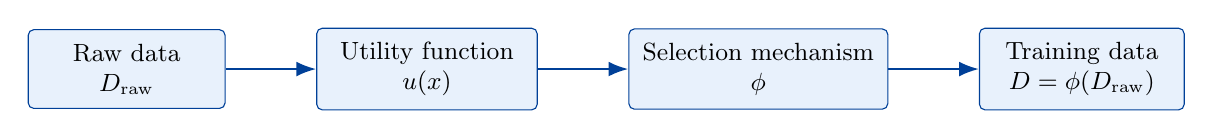
\begin{tikzpicture}[node distance=1.15cm]
  \node[methodbox, minimum width=2.5cm, minimum height=1.0cm] (raw) {Raw data\\$D_{\mathrm{raw}}$};
  \node[methodbox, minimum width=2.8cm, minimum height=1.0cm, right=of raw] (util) {Utility function\\$u(x)$};
  \node[methodbox, minimum width=3.0cm, minimum height=1.0cm, right=of util] (select) {Selection mechanism\\$\phi$};
  \node[methodbox, minimum width=2.6cm, minimum height=1.0cm, right=of select] (final) {Training data\\$D=\phi(D_{\mathrm{raw}})$};

  \draw[methodarrow] (raw) -- (util);
  \draw[methodarrow] (util) -- (select);
  \draw[methodarrow] (select) -- (final);
\end{tikzpicture}
}
\end{center}

\vspace{0.7em}

\begin{columns}[T]
\begin{column}{0.48\textwidth}
\textbf{Utility examples}
\begin{itemize}
  \item language probability
  \item quality score
  \item domain similarity
  \item duplication / toxicity score
\end{itemize}
\end{column}
\begin{column}{0.48\textwidth}
\textbf{Selection actions}
\begin{itemize}
  \item keep or remove
  \item clean part of a sample
  \item upsample or downsample
  \item reorder or select examples
\end{itemize}
\end{column}
\end{columns}

\vspace{0.3em}
\footnotesize\textit{Presenter cue: use this slide to explain that most methods share the same ``score then act'' structure.}

\end{frame}
% SOURCE: Section 2.2, original text "all data selection methods define a utility function ... as well as a selection mechanism..."

% =====================================================================
% Changxin - Methods Slide 2
% =====================================================================
\begin{frame}{Method Taxonomy: Three Questions to Ask}

\begin{columns}[T,totalwidth=\textwidth]

\begin{column}{0.32\textwidth}
\begin{block}{1. What is the goal?}
\begin{itemize}
  \item \textbf{Distribution matching}
  \item Select data similar to a desired target distribution
  \item Example: English, legal, medical, high-quality text
\end{itemize}
\end{block}
\end{column}

\begin{column}{0.32\textwidth}
\begin{block}{2. What is changed?}
\begin{itemize}
  \item \textbf{Dataset distribution}
  \item Keep, remove, or resample examples
  \item \textbf{Data point}
  \item Clean spans inside an example
\end{itemize}
\end{block}
\end{column}

\begin{column}{0.32\textwidth}
\begin{block}{3. What is the output?}
\begin{itemize}
  \item \textbf{Binary filtering}
  \item $x$ is included or removed
  \item \textbf{Weighted sampling}
  \item $x$ or a domain is sampled more or less often
\end{itemize}
\end{block}
\end{column}

\end{columns}

\vspace{0.8em}

\begin{center}
\begin{tabular}{lll}
\toprule
\textbf{Method family} & \textbf{Typical goal} & \textbf{Typical action} \\
\midrule
Language / quality filtering & distribution matching & remove examples \\
Deduplication & diversification & remove redundant data \\
Data mixing & distribution control & change sampling weights \\
Alignment selection & preference matching & rank or reweight responses \\
\bottomrule
\end{tabular}
\end{center}

\end{frame}
% SOURCE: Sections 2.3.1-2.3.4 and Table 1, which define distribution matching, diversification, dataset/data-point changes, binary vs natural-number selection, and training stages.

% =====================================================================
% Changxin - Methods Slide 3
% =====================================================================
\begin{frame}{Pretraining Pipeline: From Cheap Filters to Expensive Selection}

\begin{center}
\resizebox{\textwidth}{!}{%
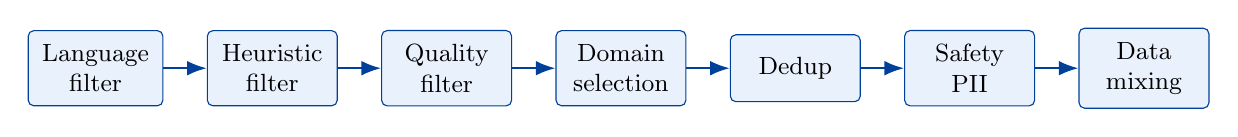
\begin{tikzpicture}[node distance=0.55cm]
  \node[methodbox, minimum width=1.65cm, minimum height=0.85cm] (lang) {Language\\filter};
  \node[methodbox, minimum width=1.65cm, minimum height=0.85cm, right=of lang] (heur) {Heuristic\\filter};
  \node[methodbox, minimum width=1.65cm, minimum height=0.85cm, right=of heur] (qual) {Quality\\filter};
  \node[methodbox, minimum width=1.65cm, minimum height=0.85cm, right=of qual] (domain) {Domain\\selection};
  \node[methodbox, minimum width=1.65cm, minimum height=0.85cm, right=of domain] (dedup) {Dedup};
  \node[methodbox, minimum width=1.65cm, minimum height=0.85cm, right=of dedup] (safe) {Safety\\PII};
  \node[methodbox, minimum width=1.65cm, minimum height=0.85cm, right=of safe] (mix) {Data\\mixing};

  \draw[methodarrow] (lang) -- (heur);
  \draw[methodarrow] (heur) -- (qual);
  \draw[methodarrow] (qual) -- (domain);
  \draw[methodarrow] (domain) -- (dedup);
  \draw[methodarrow] (dedup) -- (safe);
  \draw[methodarrow] (safe) -- (mix);
\end{tikzpicture}
}
\end{center}

\vspace{0.8em}

\begin{columns}[T]
\begin{column}{0.48\textwidth}
\textbf{Why this order?}
\begin{itemize}
  \item Raw corpora are huge, so early filters must be fast.
  \item Cheap filters remove obvious noise before expensive model-based methods.
  \item Later methods can be more targeted because fewer candidates remain.
\end{itemize}
\end{column}
\begin{column}{0.48\textwidth}
\textbf{Important caveat}
\begin{itemize}
  \item The order is a common pattern, not a universal law.
  \item Different models and domains may change the pipeline.
  \item Filter thresholds depend on the desired final token budget.
\end{itemize}
\end{column}
\end{columns}

\end{frame}
% SOURCE: Section 3 and Figure 4, original text "a common first step ... remove data with various filters" and "different works employ different filters, at different stages..."

% =====================================================================
% Changxin - Methods Slide 4
% =====================================================================
\begin{frame}{Heuristic Filters: Fast Signals for Obvious Noise}

\begin{center}
\begin{tabular}{p{0.22\textwidth}p{0.37\textwidth}p{0.30\textwidth}}
\toprule
\textbf{Heuristic family} & \textbf{Utility signal} & \textbf{Example action} \\
\midrule
Item count & number of characters, words, lines, sentences & remove documents with too few words \\
Repetition count & repeated characters, words, n-grams, lines & remove repeated boilerplate or loops \\
Existence & whether a word, phrase, or punctuation pattern appears & remove login prompts or blocked phrases \\
Ratio & alphabetic, numeric, uppercase, or symbol ratio & remove non-language or malformed text \\
Statistics & mean line length or line-length variance & flag abnormal web pages or code files \\
\bottomrule
\end{tabular}
\end{center}

\vspace{0.7em}

\begin{alertblock}{Key limitation}
Heuristics are not truth detectors. They encode assumptions about the evaluation distribution and can over-filter useful legal, medical, identity-related, or multilingual data.
\end{alertblock}

\end{frame}
% SOURCE: Section 3.2 and Table 2, which list item count, repetition count, existence, ratio, and statistics as common heuristic utility functions.

% =====================================================================
% Changxin - Methods Slide 5
% =====================================================================
\begin{frame}{Quality and Domain Filters: Matching a Target Distribution}

\begin{columns}[T,totalwidth=\textwidth]

\begin{column}{0.32\textwidth}
\begin{block}{Classifier-based quality}
\begin{itemize}
  \item Positive class: known high-quality corpora
  \item Negative class: raw web text
  \item Utility: probability of being reference-like
\end{itemize}
\end{block}
\end{column}

\begin{column}{0.32\textwidth}
\begin{block}{Perplexity-based quality}
\begin{itemize}
  \item Train an n-gram or small LM on reference text
  \item Score candidate documents
  \item Low perplexity means closer to reference data
\end{itemize}
\end{block}
\end{column}

\begin{column}{0.32\textwidth}
\begin{block}{Domain-specific selection}
\begin{itemize}
  \item Use in-domain and general-domain models
  \item Keep data that is more likely under the target domain
  \item Moore-Lewis style scoring
\end{itemize}
\end{block}
\end{column}

\end{columns}

\vspace{0.9em}

\begin{center}
\large
\[
u(x) \approx \log P(x \mid \text{target}) - \log P(x \mid \text{general})
\]
\end{center}

\vspace{-0.4em}
\footnotesize\textit{Presenter cue: explain that this is still ``score then filter,'' but the score now comes from a target distribution proxy.}

\end{frame}
% SOURCE: Sections 3.3 and 3.4, including classifier-based quality filtering, perplexity-based quality filtering, and Moore-Lewis domain selection.

% =====================================================================
% Changxin - Methods Slide 6
% =====================================================================
\begin{frame}{Deduplication: Remove Redundancy Without Killing Useful Memory}

\begin{columns}[T,totalwidth=\textwidth]

\begin{column}{0.58\textwidth}
\textbf{Common deduplication utilities}
\begin{itemize}
  \item \textbf{URL deduplication}: cheap first pass for web data
  \item \textbf{Exact hash matching}: detect identical documents
  \item \textbf{Exact substring search}: detect long copied spans
  \item \textbf{MinHash / LSH}: detect near duplicates
  \item \textbf{Model-based semantic deduplication}: detect meaning-level redundancy
\end{itemize}
\end{column}

\begin{column}{0.38\textwidth}
\begin{block}{Why it matters}
\begin{itemize}
  \item reduces training waste
  \item increases distribution coverage
  \item lowers memorization risk
  \item helps prevent test contamination
\end{itemize}
\end{block}

\begin{alertblock}{Tradeoff}
Some memorization is useful for facts, APIs, and syntax. The goal is to reduce harmful memorization, not erase all repetition.
\end{alertblock}
\end{column}

\end{columns}

\end{frame}
% SOURCE: Sections 3.5 and 10.2, including URL/hash/string/model deduplication and the discussion of memorization vs generalization.

% =====================================================================
% Changxin - Methods Slide 7
% =====================================================================
\begin{frame}{Toxicity, Explicit Content, and PII Filters}

\begin{columns}[T,totalwidth=\textwidth]

\begin{column}{0.50\textwidth}
\textbf{Common filtering mechanisms}
\begin{itemize}
  \item URL or domain blocklists
  \item lexicon / keyword matching
  \item toxicity or NSFW classifiers
  \item models trained on undesirable content
  \item regex or classifiers for PII and secrets
\end{itemize}
\end{column}

\begin{column}{0.45\textwidth}
\begin{alertblock}{No free lunch}
\begin{itemize}
  \item Toxicity filters can reduce toxic generations.
  \item But they may also remove useful examples for detecting toxic content.
  \item They may disproportionately remove text from certain communities or topics.
\end{itemize}
\end{alertblock}
\end{column}

\end{columns}

\vspace{0.5em}

\begin{center}
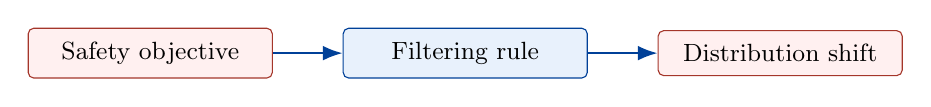
\begin{tikzpicture}
  \node[riskbox, minimum width=3.1cm] (a) at (0,0) {Safety objective};
  \node[methodbox, minimum width=3.1cm] (b) at (4,0) {Filtering rule};
  \node[riskbox, minimum width=3.1cm] (c) at (8,0) {Distribution shift};
  \draw[methodarrow] (a) -- (b);
  \draw[methodarrow] (b) -- (c);
\end{tikzpicture}
\end{center}

\end{frame}
% SOURCE: Section 3.6 and Section 10.3, especially the discussion that toxicity filtering can reduce toxic text but also reduce the model's ability to detect toxic content.

% =====================================================================
% Changxin - Methods Slide 8
% =====================================================================
\begin{frame}{Multilingual Selection: Same Pipeline, Different Parameters}

\begin{columns}[T,totalwidth=\textwidth]

\begin{column}{0.49\textwidth}
\textbf{What can be reused?}
\begin{itemize}
  \item language identification
  \item deduplication
  \item technical-character heuristics
  \item data mixing across languages
\end{itemize}
\end{column}

\begin{column}{0.49\textwidth}
\textbf{What must be adapted?}
\begin{itemize}
  \item length thresholds by language
  \item script and encoding filters
  \item language-ID confidence thresholds
  \item native-speaker quality checks for low-resource languages
\end{itemize}
\end{column}

\end{columns}

\vspace{0.8em}

\begin{block}{Example intuition}
Chinese can carry more information per character than English, so an English minimum-length threshold may incorrectly remove useful Chinese text.
\end{block}

\vspace{0.3em}
\footnotesize\textit{Presenter cue: emphasize that multilingual filtering is not just ``run the English pipeline on every language.''}

\end{frame}
% SOURCE: Section 3.7, original text discussing language-specific filtering hyperparameters and native-speaker involvement for low-resource languages.

% =====================================================================
% Changxin - Methods Slide 9
% =====================================================================
\begin{frame}{Data Mixing: Sampling Weights Are Also Data Selection}

\textbf{When a corpus has multiple domains, data selection also decides how often each domain appears during training.}

\vspace{0.7em}

\begin{center}
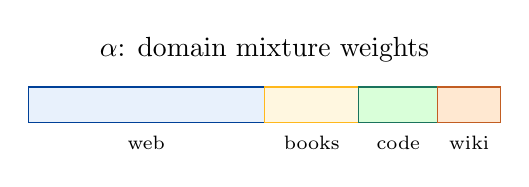
\begin{tikzpicture}
  \draw[fill=softblue, draw=ucrblue] (0,0) rectangle (3.0,0.45);
  \draw[fill=softgold, draw=ucrgold] (3.0,0) rectangle (4.2,0.45);
  \draw[fill=green!15, draw=methodgreen] (4.2,0) rectangle (5.2,0.45);
  \draw[fill=orange!18, draw=methodorange] (5.2,0) rectangle (6.0,0.45);
  \node[below] at (1.5,-0.05) {\scriptsize web};
  \node[below] at (3.6,-0.05) {\scriptsize books};
  \node[below] at (4.7,-0.05) {\scriptsize code};
  \node[below] at (5.6,-0.05) {\scriptsize wiki};
  \node[above] at (3.0,0.65) {$\alpha$: domain mixture weights};
\end{tikzpicture}
\end{center}

\vspace{0.9em}

\begin{columns}[T,totalwidth=\textwidth]
\begin{column}{0.49\textwidth}
\textbf{How weights are chosen}
\begin{itemize}
  \item natural data proportions
  \item manually chosen weights
  \item small-model empirical search
  \item principled updates such as DoReMi or DoGE
  \item online updates during training
\end{itemize}
\end{column}
\begin{column}{0.49\textwidth}
\begin{alertblock}{Core tradeoff}
Upweighting one source necessarily downweights others under a fixed training budget. Good weights may not transfer across tokenizer, model scale, or training length.
\end{alertblock}
\end{column}
\end{columns}

\end{frame}
% SOURCE: Section 3.8, including domain weights, heuristic/manual/empirical/principled approaches, DoReMi, DoGE, online data mixing, and transfer challenges.

% =====================================================================
% Changxin - Methods Slide 10
% =====================================================================
\begin{frame}{Beyond Pretraining: Instruction Tuning and Alignment}

\begin{columns}[T,totalwidth=\textwidth]

\begin{column}{0.48\textwidth}
\begin{block}{Instruction tuning}
\textbf{Data format:} instruction $\rightarrow$ output
\begin{itemize}
  \item diversify tasks and user intents
  \item unify task formats
  \item generate synthetic instructions
  \item select high-quality / complex / diverse examples
\end{itemize}
\end{block}
\end{column}

\begin{column}{0.48\textwidth}
\begin{block}{Preference fine-tuning}
\textbf{Data format:} prompt + chosen + rejected
\begin{itemize}
  \item manual filtering
  \item model-based evaluation
  \item reward-model reweighting
  \item rejection sampling / best-of-$N$
\end{itemize}
\end{block}
\end{column}

\end{columns}

\vspace{0.8em}

\begin{alertblock}{Important distinction}
Pretraining selection often optimizes broad coverage and efficiency; alignment selection optimizes qualitative preferences such as helpfulness and harmlessness.
\end{alertblock}

\end{frame}
% SOURCE: Sections 4 and 5, covering instruction-tuning diversification, synthetic instruction data, preference fine-tuning, reward models, and rejection sampling.

% =====================================================================
% Changxin - Methods Slide 11
% =====================================================================
\begin{frame}{Practical Recipe for Choosing a Method}

\begin{enumerate}
  \item \textbf{Define the target distribution.}
  General LLM, code model, domain model, assistant model, or task-specific model?

  \item \textbf{Choose the objective.}
  Model performance, data efficiency, evaluation integrity, safety, or selection efficiency?

  \item \textbf{Start with cheap filters.}
  Language, length, obvious noise, URL/hash deduplication.

  \item \textbf{Add target-aware scoring only when needed.}
  Quality classifier, perplexity, domain ratio, reward model, retriever, or gradient utility.

  \item \textbf{Audit the side effects.}
  False positives, data bias, benchmark leakage, memorization, multilingual loss.
\end{enumerate}

\vspace{0.6em}

\begin{center}
\Large\color{ucrblue}\textbf{Takeaway: data selection is training-distribution design.}
\end{center}

\end{frame}
% SOURCE: Sections 10.5 and 11, especially considerations for applying data selection and the call to better understand target distributions.





% =====================================================================
% Slide #: Divider Slide for Applications, Results, and Future
% =====================================================================
\begin{frame}

\begin{center}

\vspace{2cm}

{\color{ucrblue}\Huge\textbf{Part 3}}

\vspace{0.8cm}

{\LARGE Applications, Results, \& Future}

\vspace{1cm}

{\large Data Selection for LLMs}

\end{center}

\end{frame}

% % =====================================================================
% % Slide 4: BDX (Bank Division with XOR)
% % =====================================================================
% \begin{frame}{Methodology (1): BDX, Adding Read Ports with XOR}
%   \begin{columns}[T]
%     \begin{column}{0.52\textwidth}
%       \textbf{Bank Division with XOR (BDX)}
%       \begin{itemize}
%         \item Section III A 1, increases \textbf{read} ports
%         \item Avoids replicating the whole memory space
%         \item 4 data banks + 1 XOR bank
%         \item $P_n = D_{(0,n)} \oplus D_{(1,n)} \oplus D_{(2,n)} \oplus D_{(3,n)}$ (4)
%       \end{itemize}

%       \vspace{0.4em}
%       \textbf{Conflicting read recovery}
%       \begin{itemize}
%         \item One read accesses the bank directly
%         \item The other recovers via XOR:
%         \item $D_{(1,n)} = D_{(0,n)} \oplus D_{(2,n)} \oplus D_{(3,n)} \oplus P_n$ (5)
%       \end{itemize}

%       \vspace{0.4em}
%       \footnotesize \textit{Note: BDX uses XOR to add read ports. Different from XOR based [2], which uses XOR to add write ports.}
%     \end{column}
%     \begin{column}{0.48\textwidth}
%       \centering
%       \includegraphics[width=\linewidth]{figures1/fig6_bdx.png}
%       \footnotesize Fig.\ 6: BDX 2R1W example
%     \end{column}
%   \end{columns}
% \end{frame}

% =====================================================================
% Slide 5: 2R1W/4R Two Mode Module
% =====================================================================
% \begin{frame}{Methodology (2): 2R1W/4R, A Two Mode Memory}
%   \begin{columns}[T]
%     \begin{column}{0.52\textwidth}
%       \textbf{Key insight (Section III A 2)}
%       \begin{itemize}
%         \item Same 2R1W hardware, used as either 2R1W or 4R
%         \item Denoted as \textbf{2R1W/4R}, a hybrid module
%         \item Same design as BDX 2R1W; only the usage mode differs
%       \end{itemize}

%       \vspace{0.5em}
%       \textbf{Two operating modes}
%       \begin{itemize}
%         \item \textbf{2R1W mode}: with a write request, supports up to 2 conflicting reads
%         \item \textbf{4R mode}: no write request, supports up to 4 conflicting reads
%         \item In 4R mode, conflicts resolved via XOR on other banks + XOR bank
%       \end{itemize}
%     \end{column}
%     \begin{column}{0.48\textwidth}
%       \centering
%       \includegraphics[width=\linewidth]{figures1/fig8_2r1w4r.png}
%       \footnotesize Fig.\ 8: (a) 2R1W mode, (b) 4R mode
%     \end{column}
%   \end{columns}
% \end{frame}


% % =====================================================================
% % Slide 6: HBDX
% % =====================================================================
% \begin{frame}{Methodology (3): HBDX, Hierarchical 4R1W Design}
%   \begin{columns}[T]
%     \begin{column}{0.55\textwidth}
%       \textbf{Hierarchical Bank Division with XOR (HBDX)}
%       \begin{itemize}
%         \item Section III A 3: a 4R1W memory using 2R1W/4R as building blocks
%         \item Avoids replicating the 2R1W module
%         \item Hierarchical structure organizes 2R1W into 4R1W
%       \end{itemize}

%       \vspace{0.4em}
%       \textbf{Worst case: all 4R + 1W target bank 0}
%       \begin{itemize}
%         \item $R_0$, $R_1$ read directly from bank 0
%         \item $R_2$, $R_3$ recover via XOR on other banks + XOR bank
%         \item $W_0$ stores to bank 0; XOR bank updated in two cycle pipeline
%         \item Bank 0 in 2R1W mode, others in 4R mode
%       \end{itemize}
%     \end{column}
%     \begin{column}{0.45\textwidth}
%       \centering
%       \includegraphics[width=\linewidth]{figures1/fig9_hbdx.png}
%       \footnotesize Fig.\ 9: HBDX 4R1W
%     \end{column}
%   \end{columns}
% \end{frame}


% % =====================================================================
% % Slide 7: BDRT and Integrated Architecture
% % =====================================================================
% \begin{frame}{Methodology (4): BDRT and Integrated Architecture}
%   \begin{columns}[T]
%     \begin{column}{0.52\textwidth}
%       \textbf{Bank Division with Remap Table} (Sec. III B)
%       \begin{itemize}
%         \item Increases \textbf{write} ports
%         \item Avoids replicating whole memory (unlike LVT)
%         \item Bank buffers + remap table track latest data
%         \item Smaller storage than LVT
%       \end{itemize}

%       \vspace{0.4em}
%       \textbf{Integrated mRnW architecture} (Sec. III C)
%       \begin{itemize}
%         \item HBDX (multi read) + BDRT (multi write)
%         \item $k$ data banks + $(n-1)$ bank buffers
%         \item Hash mechanism distributes writes
%       \end{itemize}
%     \end{column}
%     \begin{column}{0.48\textwidth}
%       \centering
%       \includegraphics[width=\linewidth]{figures1/fig11_integrated.png}
%       \footnotesize Fig.\ 11: HBDX + BDRT integrated
%     \end{column}
%   \end{columns}
% \end{frame}

% % =====================================================================
% % Slide 8: Evaluation Setup
% % =====================================================================
% \begin{frame}{Evaluation Setup}
%   \textbf{FPGA platform} (Section IV A)
%   \begin{itemize}
%     \item Xilinx Virtex 7 XC7V585 FPGA
%     \item 795 BRAMs, 91{,}050 slices available
%     \item Each BRAM: 32 bit data width by 1K depth
%     \item Design tool: Xilinx ISE 14.2 (synthesis set to favor clock frequency)
%   \end{itemize}

%   \vspace{0.5em}
%   \textbf{Designs compared}
%   \begin{itemize}
%     \item LVT based, XOR based (prior work)
%     \item LVT based + BDX, LVT based + HBDX
%     \item XOR based + BDX, XOR based + HBDX
%     \item BDRT based, BDRT based + 2R1W/4R (proposed)
%   \end{itemize}

%   \vspace{0.3em}
%   \textbf{Metrics}: number of BRAMs, operating frequency, slice utilization
% \end{frame}

% % =====================================================================
% % Slide 9: Results, 4R2W and 4R3W
% % =====================================================================
% \begin{frame}{Results: 4R2W and 4R3W Memory}
%   \begin{columns}[T]
%     \begin{column}{0.42\textwidth}
%       \textbf{4R2W with 8K depth (Table III)}
%       \begin{itemize}
%         \item BDX/HBDX: 30 to 53\% fewer BRAMs
%         \item BDRT based: up to 69\% fewer BRAMs vs LVT based
%         \item Tradeoff: BDRT based runs 16 to 19\% slower
%       \end{itemize}
 
%       \vspace{0.4em}
%       \textbf{4R3W with 8K depth (Table IV)}
%       \begin{itemize}
%         \item XOR based + BDX/HBDX: 37.5 / 48\% fewer BRAMs, +13\% freq
%         \item LVT based + BDX/HBDX: 37.5 to 53\% fewer BRAMs, +20\% freq
%       \end{itemize}
%     \end{column}
%     \begin{column}{0.58\textwidth}
%       \centering
%       \includegraphics[width=0.92\linewidth]{figures1/table3_4r2w_results.png}\\
%       {\scriptsize Table III: 4R2W performance}
 
%       \vspace{0.4em}
%       \includegraphics[width=0.92\linewidth]{figures1/table4_4r3w_results.png}\\
%       {\scriptsize Table IV: 4R3W performance}
%     \end{column}
%   \end{columns}
% \end{frame}
% %=====================================================================
% % Slide 10: Bank Organization
% % =====================================================================
% \begin{frame}{Impact of Bank Organization}
%   \textbf{Tuning the bank organization} (Section IV E, Table V)
%   \begin{itemize}
%     \item Studied design: BDRT based + 2R1W/4R for 4R3W memory with 8K depth
%     \item Compared two configurations:
%     \begin{itemize}
%       \item 2 data banks + 3 bank buffers (5 banks total)
%       \item 4 data banks + 3 bank buffers (7 banks total)
%     \end{itemize}
%     \item Each bank's depth shrinks from 4K to 2K when going from 2 banks to 4 banks
%   \end{itemize}

%   \vspace{0.5em}
%   \textbf{Results: 4 data bank vs 2 data bank}
%   \begin{itemize}
%     \item BRAM usage: down by 16 percent
%     \item Frequency: up by 21 percent
%     \item Slice utilization: down by 27 percent
%   \end{itemize}

%   \vspace{0.3em}
%   \textit{$\rightarrow$ Bank organization is a promising direction for further design refinement (the authors mark it as future work).}
% \end{frame}


% % =====================================================================
% % Slide 11: Conclusion + Class Relations + Comments
% % =====================================================================
% \begin{frame}{Conclusion, Class Relations, and Comments}
%   \textbf{Summary of contributions} (Section V)
%   \begin{itemize}
%     \item Novel 2R1W/4R: same hardware, two usage modes
%     \item HBDX 4R1W: up to 33 percent fewer BRAMs than replication
%     \item For 4R3W with 8K depth: 53 percent fewer BRAMs, 20 percent higher frequency
%   \end{itemize}

%   \vspace{0.3em}
%   \textbf{How this paper relates to CS 220}
%   \begin{itemize}
%     \item RTL modeling and synthesis (Weeks 2 to 3); Memory design (Weeks 6 to 7)
%     \item Same philosophy as our project: reuse existing hardware to gain more functionality
%   \end{itemize}

%   \vspace{0.3em}
%   \textbf{Our comments}
%   \begin{itemize}
%     \item Abstract claims 25 percent BRAM reduction; Conclusion says 33 percent. Inconsistency
%     \item BDRT based + 2R1W/4R cannot synthesize at 4R3W 16K depth
%     \item Authors acknowledge: writes still need table lookup, room for future work
%   \end{itemize}
% \end{frame}


\end{document}
